\documentclass[tikz]{standalone}

\definecolor{NewHex}{HTML}{648FFF}

\begin{document}
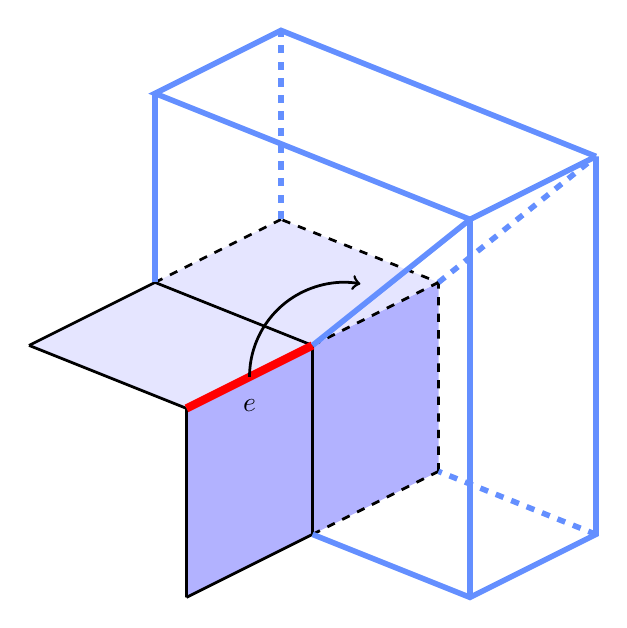
\begin{tikzpicture}[scale=4, x={(0.5cm,-0.2cm)}, y={(0.4cm,0.2cm)}, z={(0.0cm,0.6cm)}]

  %%%%%%%%%% Points pour travailler %%%%%%%%%%
 \coordinate (0) at (0,0,0);
 \coordinate (1) at (0,1,0);
 \coordinate (2) at (0,2,0);
 \coordinate (4) at (0,0,1);
 \coordinate (5) at (0,1,1);
 \coordinate (6) at (0,2,1);
 \coordinate (8) at (1,1,1);
 \coordinate (9) at (1,2,1);
 \coordinate (10) at (-1,0,1);
 \coordinate (11) at (-1,1,1);
 \coordinate (12) at (-1,2,1);
 \coordinate (14) at (0,1,2);
 \coordinate (15) at (0,2,2);
 \coordinate (16) at (1,1,2);
 \coordinate (17) at (1,2,2);

 \coordinate (18) at (1,1,0);
 \coordinate (19) at (1,2,0);
 \coordinate (20) at (-1,1,2);
 \coordinate (21) at (-1,2,2);

 %%%%%%%%%% Layer blue color %%%%%%%%%%
 \fill [color=blue!30!white] (4) -- (6) -- (2) -- (0) -- cycle ;
 \fill [color=blue!10!white] (4) -- (6) -- (12) -- (10) -- cycle ;
 
 % Layer 1
 \draw [line width=1] (0) -- (1) ;
 \draw [dashed, line width=1] (1) -- (2) ;
 \draw [line width=1] (4) -- (5) ;
 \draw [dashed, line width=1] (5) -- (6) ;
 \draw [line width=1] (10) -- (11) ;
 \draw [dashed, line width=1] (11) -- (12) ;
 
 \draw [line width=1] (0) -- (4) -- (10) ;
 \draw [line width=1] (1) -- (5) -- (11) ;
 \draw [dashed, line width=1] (2) -- (6) -- (12) ;

 \draw [line width=3, color=red] (4) -- (5) ;

 % Hexa 2
 \draw [line width=2, color=NewHex] (16) -- (17) ;
 \draw [line width=2, color=NewHex] (5) -- (16) ;
 \draw [dashed, line width=2, color=NewHex] (6) -- (17) ;
 \draw [line width=2, color=NewHex] (11) -- (20) ;
 \draw [line width=2, color=NewHex] (16) -- (20) -- (21) -- (17) ;
 \draw [dashed, line width=2, color=NewHex] (12) -- (21) ;

 % Hexa 3
 \draw [line width=2, color=NewHex] (16) -- (18) ;
 \draw [line width=2, color=NewHex] (1) -- (18) -- (19) -- (17) ;
 \draw [dashed, line width=2, color=NewHex] (19) -- (2) ;

 %\foreach \i in {0,...,17}
 %{
 %  \draw (\i) node[circle, fill=black, inner sep = 2 pt] {};
 %}

 \draw (0,0.5,0.85) node[color=black, scale=1] (edge) {$e$} ;
 \draw[->, line width=1] (0,0.5,1) arc (180:80:0.3cm);


\end{tikzpicture}
\end{document}